\documentclass{report}
\usepackage[T1]{fontenc} % Fontes T1
\usepackage[utf8]{inputenc} % Input UTF8
\usepackage[backend=biber, style=ieee]{biblatex} % para usar bibliografia
\usepackage{csquotes}
\usepackage[portuguese]{babel} %Usar língua portuguesa
\usepackage{blindtext} % Gerar texto automaticamente
\usepackage[printonlyused]{acronym}
\usepackage{hyperref} % para autoref
\usepackage{graphicx}
\usepackage{indentfirst}

\bibliography{bibliografia}



\begin{document}
%%
% Definições
%

\def\titulo{Energias}
\def\data{DATA}
\def\autores{Francisco Franco, Tomás Oliveira}
\def\autorescontactos{(113275) franco.f04@ua.pt, (113939) tomas.esteves.oliveira@ua.pt}
\def\versao{VERSAO 1}
\def\departamento{Dept. de Eletrónica, Telecomunicações e Informática}
\def\empresa{Universidade de Aveiro}
\def\logotipo{ua.pdf}
%
%%%%%% CAPA %%%%%%
%
\begin{titlepage}

\begin{center}
%
\vspace*{50mm}
%
{\Huge \ Energias}\\ 
%
\vspace{10mm}
%
{\Large \empresa}\\
%
\vspace{10mm}
%
{\LARGE \autores}\\ 
%
\vspace{30mm}
%
\begin{figure}[h]
\center
\includegraphics{\logotipo}
\end{figure}
%
\vspace{30mm}
\end{center}
%
\begin{flushright}
\versao
\end{flushright}
\end{titlepage}

%%  Página de Título %%
\title{%
{\Huge\textbf{\titulo}}\\
{\Large \departamento\\ \empresa}
}
%
\author{%
    \autores \\
    \autorescontactos
}
%
\date{\today}
%
\maketitle
\pagenumbering{roman}

%%%%%% RESUMO %%%%%%
\begin{abstract}
Neste projeto decidimos começar por decidir qual o tema iriamos abordar. Acabamos assim por optar pelas Energias devido à grande consideração e relevância que ambos atribuímos a esta temática. Este tópico é bastante comum de ser apresentado, mas não achamos que deva ser excluído por causa disso. O trabalho foi feito maioritariamente de forma distanciada, utilizando métodos que nos foram introduzidos na unidade curricular de IEI, em que a cada elemento do grupo foram atribuídas tarefas tendo sido devidamente executadas com sucesso. Concluindo queremos reforçar que através da realização desta atividade foi compreendido pela nossa parte o quão importante estas energias são para o normal funcionamento da sociedade visto que nada acontece sem esta energia que constitui este nosso Universo. Algo que nos conquistou bastante também foi a rápida evolução da humanidade na utilização destas Energias já que no século XX eram apenas utilizadas energias não renováveis, bastante prejudiciais para o nosso planeta devido à poluição. Ao contrário do seculo XXI que irá beneficiar as energias não renováveis que terá fortes impactos positivos no meio ambiente para além destas serem inesgotáveis. 
\end{abstract}

%%%%%% Agradecimentos %%%%%%
% Segundo glisc deveria aparecer após conclusão...
\renewcommand{\abstractname}{Agradecimentos}
\begin{abstract}
Gostaríamos de agradecer, de uma forma breve, ao nosso professor desta unidade curricular António Manuel Adrego da Rocha pela maneira cativante como ensina os alunos durante as aulas de modo a obtermos as melhores técnicas/ferramentas para executar os trabalhos que nos forem propostos.
“Ser professor não é só uma questão de possuir um corpo de
conhecimentos e capacidade de controlo da aula. Isso
poderia fazer-se com um computador e um bastão. Para ser
professor é preciso, igualmente, ter capacidade de
estabelecer relações humanas com as pessoas a quem se
ensina. Aprender é um processo social humano e árduo, o
mesmo se pode dizer de ensinar. Ensinar implica,
simultaneamente, emoções e razão pura". 
\end{abstract}


\tableofcontents
% \listoftables     % descomentar se necessário
% \listoffigures    % descomentar se necessário


%%%%%%%%%%%%%%%%%%%%%%%%%%%%%%%
\clearpage
\pagenumbering{arabic}

%%%%%%%%%%%%%%%%%%%%%%%%%%%%%%%%
\chapter{Introdução}
\label{chap.introducao}
No âmbito do relatório técnico da unidade curricular de IEI (Introdução à Engenharia informática) foi-nos atribuída a exploração de um tema à nossa escolha e decidimos optar pelas Energias. Neste trabalho iremos explicar, de uma maneira clara e objetiva o que são Energias bem como a sua contextualização na sociedade, referir as vantagens e algumas desvantagens que estas trazem para a sociedade. Iremos também apresentar os principais tipos de energias. Consideramos que falar sobre este tema é indispensável, especialmente nos dias de hoje devido à guerra, pois estas energias renováveis são recursos inesgotáveis e evitam que Portugal seja dependente de outros países devido à importação de combustíveis fósseis, como é o caso do carvão e/ou o gás natural.

\begin{center}
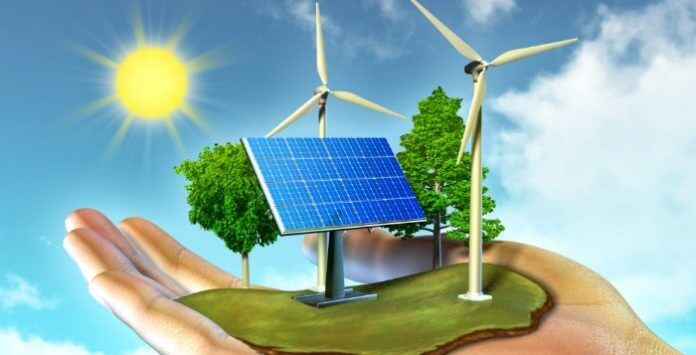
\includegraphics[width=10cm]{Trabalho IEI/fontes.jpg}
\end{center}

\label{chap.metodologia}


\chapter{Contextualização das Energias}
Relativamente à história da humanidade e da energia muitas vezes temos dificuldade em saber quem foi o impulsionador de quem. No entanto, sabemos que uma delas influenciou bastante o desenvolvimento da outra. Ao longo da história é possível identificar este desenvolvimento, visto que a humanidade teve a capacidade de progredir utilizando a energia. Iremos apresentar os principais acontecimentos da energia no passado e as perspetivas futuras da mesma.

Num primeiro momento, á muito tempo atrás, a maneira como o ser humano utiliza energia e as formas para as obter foram se alterando ao longo do tempo, tendo uma influência indispensável no modo como vivemos. No início, eram apenas utilizadas as energias obtidas de alimentos para a realização de tarefas do quotidiano, como é o caso da caça e o desenvolvimento de instrumentos que tornassem esta atividade tão importante na altura mais eficiente. Quando surgiu o fogo, foi possível ter-se um melhor aproveitamento dos alimentos e houve uma melhoria na qualidade de vida, visto que houve um decréscimo relativamente ao risco de apanhar doenças ou até mesmo alguma infeção presente nos alimentos. Caso bastante comum naquele tempo já que os alimentos não estavam devidamente cozinhados.  Durante bastante tempo, o uso da energia limitou-se apenas à energia obtida através dos alimentos e/ou queima de combustíveis, até que se passou a utilizar a energia dos animais de modo a uma realização de atividades diárias mais eficaz, o que causou um aumento da capacidade de produção da comunidade em geral, permitindo ainda o aparecimento de novas atividades como é o caso da escrita, do artesanato, e da engenharia. Um outro grande avanço na história da humanidade foi o desenvolvimento de barco á vela. Deste modo era utilizado a energia dos ventos e consequentemente houve a possibilidade de nos deslocarmos por grandes distâncias num espaço de tempo mais curto. Esta técnica foi inicialmente criada pelos fenícios. Cada vez mais significantes passaram a ser estas energias já que por volta de 1698 surgiu a primeira máquina a vapor que servia inicialmente para tirar água dos poços de minas de carvão. Já para não falar dos primeiros carros a vapor agilizando alguns processos como por exemplo o deslocamento muito mais rápido de pessoas, o que teve uma influência grande relativamente aos preços dos produtos daquela época. Apesar de todas estas evoluções incríveis na nossa sociedade não nos podemos esquecer da mais importante e que mais veio revolucionar o mundo em que vivemos. Referimo-nos, portanto, á energia elétrica descoberta em 1879 inicialmente utilizada para meios de comunicação, entretenimento e iluminação para além de muitos outros aspetos. Realçamos também que com a evolução da tecnologia esta energia elétrica pode ser transmitida através de fios por várias centenas de quilómetros de distância.

A época atual é facilmente caracterizada pelo uso abundante da energia e pela procura de novas fontes dessa. No presente a energia deixou de ser utilizada apenas para preparação de alimentos e iluminação.  As evoluções foram tais que nos dias de hoje utilizamos energia para praticamente tudo, incluindo transportes e comunicação. 
Expandiram-se assim diversas formas de produção de energia que vamos explicitar mais à frente.



\chapter{Qual a Importância da Energia}
A energia é um bem indispensável, pois facilita o quotidiano das populações e é utilizada para quase todas as tarefas diárias e hoje em dia torna-se impossível imaginar a vida moderna sem essa mesma energia, pelo facto de necessitarmos dela em quase todas as nossas atividades diárias. Visto que a eletricidade é fundamental nos moldes da nossa sociedade atual, onde nos fornece o conforto, bem-estar, segurança e lazer para a sociedade.
Essa energia nem sempre  é utilizada de maneira correta, devido a um consumo excessivo, que pode ser evitado ao diminuirmos o uso de aparelhos que nem sempre são necessários. 



\chapter{Energias Renováveis}
\section{O que são as Energias Renováveis}
O termo renovável demonstra que algo, nomeadamente uma energia, está disponível na natureza e tem a habilidade de se regenerar continuamente, em quantidades praticamente inesgotáveis. Por assim dizer estas energias provêm de recursos naturais que não têm limites daí a importantíssima razão para as utilizarmos.



\section{Principais tipos de Energias Renováveis}
Diferentes tipos de Energias Renováveis correspondem ás maneiras pelas quais podemos, devido aos avanços tecnológicos, produzir energia através de distintas fontes naturais. Neste trabalho iremos abordar apenas as principais métodos como por exemplo pelo meio solar, eólico e finalmente hidráulico.



\subsection{Energia Solar}

A energia solar é a energia proveniente da luz e do calor do Sol, sendo a que tem menor impacto ambiental. É uma excelente forma de obter energia limpa e sustentável sem danificar o meio ambiente. Atualmente são aplicadas diversas tecnologias de modo a este tipo de energias serem úteis na vida dos seres humanos como é o caso dos painéis solares que são cruciais para o aquecimento da água usada no dia a dia como é o caso de piscinas ou simplesmente para tomar um duche.

\begin{center}
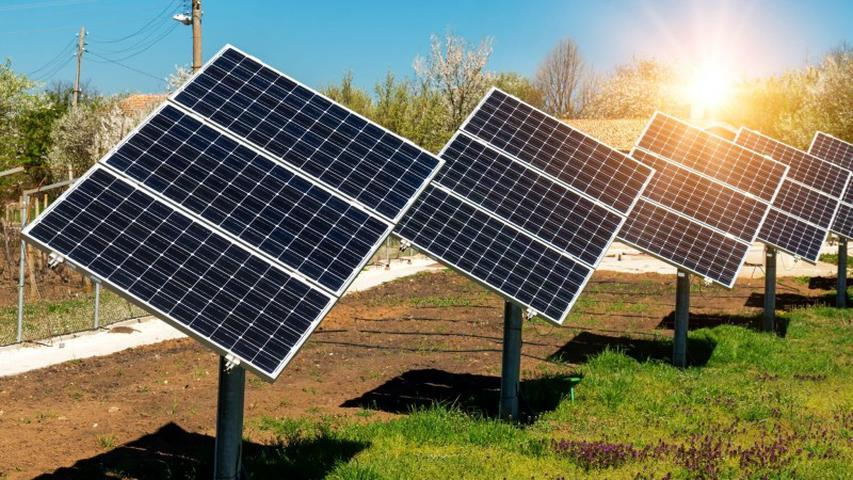
\includegraphics[width=8cm]{energia solar.jpeg}
\end{center}

\subsection{Energia Eólica}
A utilização da energia eólica não é recente, remonta a épocas em que a força do vento já era usada para mover barcos à vela, bombear água e moer grãos. Mas atualmente tem cada vez mais impacto e pode, de facto, mover o mundo no sentido da sustentabilidade. Principalmente num tempo em que se discute a escassez de recursos energéticos e urge a preocupação com as mudanças climáticas, uma aposta mais forte em energias renováveis, como a utilização do vento, um recurso inesgotável e natural, é crucial para a transição energética e para a construção de um futuro melhor.
Esta obtém-se a partir da força do vento, através de uma turbina eólica, ou aerogerador. Este equipamento aproveita a energia do vento e converte-a em energia elétrica. Normalmente para tirar mais proveito desta energia, as eólicas são colocadas onde existe uma maior intensidade de vento. 
Estas eólicas têm em média entre 80 e 120 metros de altura e estão orientadas na direção do vento, depois esta força é captada e a energia mecânica da rotação é convertida em energia elétrica, depois a energia produzida é transportada por cabos subterrâneos até uma subestação de transformação para que possa assim ser distribuída. 


\begin{center}
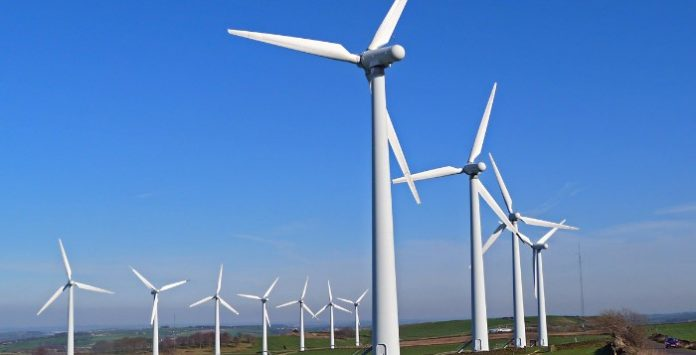
\includegraphics[width=8cm]{parque-eolico5.jpeg}
\end{center}

\subsection{Energia Hidráulica}
A energia hidráulica é obtida através da energia da água, ou seja, a forma pela qual esta se manifesta na natureza é nos fluxos de água, como rios e lagos e é também utilizada por meio da queda de água. Pode ser convertida na forma de energia mecânica através de ferramentas desenvolvidas como é o caso de turbinas hidráulicas ou moinhos de água. As turbinas podem ser usadas como acionamento de um equipamento industrial, como um compressor, ou de um gerador elétrico, com a finalidade de prover energia elétrica para uma rede de energia.


\begin{center}
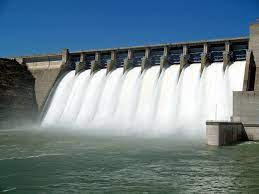
\includegraphics[width=8cm]{energia hidrica.jpeg}
\end{center}


\subsection{Energia Geotérmica}
A energia geotérmica, utiliza o calor proveniente do interior da terra, primeiro perfura-se em locais com uma grande quantidade de vapor de água acumulado por este calor, este irá posteriormente ser levado até à superfície através de tabulagem específica, esta irá girar uma turbina criando energia elétrica. As maiores desvantagens apontadas a esta energia são ser uma energia muito cara e pouco rentável, a emissão de substâncias e calor para a ambiente.


\begin{center}
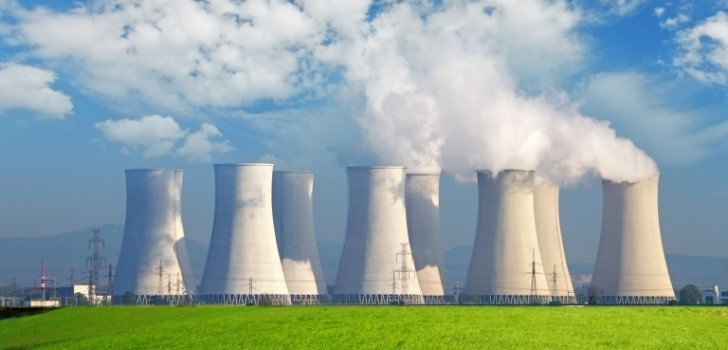
\includegraphics[width=8cm]{energia-nuclear.jpg}
\end{center}


\section{Utilização de Energias Renováveis em Portugal}
Portugal apresenta valores impressionantes relativamente ao uso destas energias visto que fomos reconhecidos, em 2019, como o quarto país da Europa com a maior inclusão de energias renováveis na produção de eletricidade. Neste ano, segundo os dados da empresa Redes Energéticas Nacionais, por volta de metade da energia usada pelo nosso país foi renovável tendo assim ultrapassando os valores das energias não renováveis passando estas a serem utilizadas menos de metade do total de energias. Os valores restantes representam os consumos energético importados podendo ser, ou não, renováveis. Os países a nossa frente foram a Dinamarca, Áustria e a Suécia como apresentado na figura 4.1.



Portugal, nos últimos anos tem tido uma prestação excelente relativamente ao uso destas energias e é expectável que este alcance a meta para 2030 já em 2025 no que diz respeito à produção de energia via fontes renováveis como é o caso da energia solar. A previsão é alcançar dois quintos de energia produzida a partir de energias renováveis cinco anos antes do que estava previsto. Em janeiro de 2022 mais de metade da eletricidade já veio das renováveis. O Ministro do Ambiente e da Ação Climática Duarte Cordeiro, anuncia que “Portugal tem um ponto forte nas energias renováveis e é nosso dever focarmos-mos no desenvolvimento das mesmas”.

Num cenário mais abrangente, falemos da União Europeia que, como é o caso de Portugal, estão a superar as metas definidas na produção de eletricidade através de energias renováveis. Assim os representantes da Comissão Europeia estão a ponderar aumentar as metas de energia renovável para 2030. Um dos objetivos da União Europeia é implementar uma medida de modo a tornar os painéis solares obrigatórios nos telhados de todos os novos edifícios.

\begin{table}[h]
\centering
\caption{Um nome qualquer}
\vspace{0.5cm}
\begin{tabular}{r|lr}

Posi{\c c}{\~a}o & Pa{\'i}s & (Percentagem de Energia Renovável Utilizada) \\ 
\hline                              
1 & Áustria        & 78 \\
2 & Suécia   & 72 \\
3 & Dinamarca            & 65 \\
4 & Portugal        & 51 \\
           

\end{tabular}
\end{table}

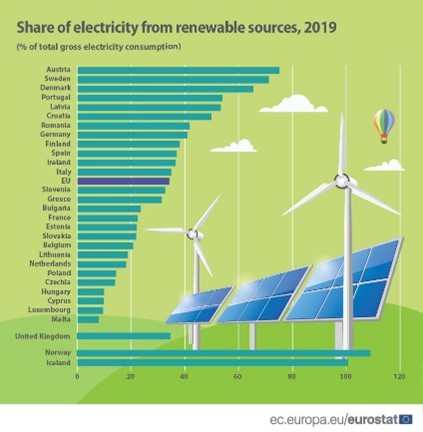
\includegraphics[width = 3cm]{Image.jpg}
\clearpage





\section{Fatores a considerar:}

\subsection{Vantagens}
Neste tópico iremos abordar algumas vantagens de cada uma destas Eneregias Renováveis.

A energia solar, é um dos exemplos de melhor energia, pois não trás qualquer tipo de dano para a natureza, e é um recurso ilimitado. Esta energia, através de painéis fotovoltaicos, transforma os raios solares em energia através de células fotovoltaicas ou de espelhos parabólicos onde o calor proveniente deste cria vapor de água o que faz girar uma turbina gerando energia elétrica. 


A energia eólica que não emite gases poluentes nem gera resíduos, pois não utiliza processos de combustão. Ao reduzir a utilização de combustíveis fósseis, diminuem as emissões de dióxido de carbono, entre outras substâncias nocivas, que modificam o clima e são responsáveis pelo efeito estufa. Para além disso, é uma energia mais barata do que outras energias, quer no custo por kW, quer na sua manutenção, em particular nos locais onde o vento é mais forte e frequente. 


A energia hidráulica utiliza uma fonte limpa e renovável, a água, onde não emite gases para a atmosfera e é uma fonte de eletricidade que fica mais econômica para o consumidor final. Para além de ser econômica, reforça também a economia com o turismo.


A energia geotérmica é “alimentada” com usinas de longa duração e tem cada vez menos riscos e mais potencial. É silenciosa, e temos acesso a esta energia sem grandes impactos paisagísticos e é bastante versátil. Também pode servir para a refrigeração e pode criar mais empregos do que qualquer outra fonte de energia verde.

\subsection{Desvantagens}

A energia solar, durante a noite não tem qualquer tipo de produção de energia, o que obriga à existência de meios de armazenamento da energia produzida durante o dia. No entanto, as formas de armazenamento desta energia são pouco eficientes, quando comparadas, por exemplo, aos combustíveis fósseis. Como podemos constatar, existem diversos tipos de produção de energia, desde os mais poluentes aos menos prejudiciais para o nosso planeta. As alterações climáticas e a inovação tecnológica criaram um novo mundo de desafios para o setor da energia: a redução urgente das emissões de CO2.

A energia eólica tem como fonte geradora o vento, que é muito irregular, então a geração de energia muitas vezes pode ser imprevisível, e os equipamentos acabam por ter um custo elevado, e para que exista uma grande produção é preciso criar um grande parque eólico para comportar as eólicas o que acaba por ser um grande impacto visual, e um grande incômodo sonoro para quem mora nos arredores.

A energia hídrica, a água armazenada em barragens cai de uma elevada altura colocando turbinas em movimento criando assim energia elétrica, as desvantagens apresentadas são durante a construção é necessário o alargamento de uma grande área, prejudicando a fauna e flora, como alteração do curso e do nível natural dos rios, diminuição da geração nos períodos de seca e a realocação das populações ribeirinhas e nativas.

A energia geotérmica, utiliza o calor proveniente do interior da terra, primeiro perfura-se em locais com uma grande quantidade de vapor de água acumulado por este calor, com estas prefurações pode existir eventual afundamento do terreno, causa poluição sonora e elevado aquecimento local, emite para atmosfera gás sulfídrico, e pode eventualmente causar uma contaminaçao de rios e lagos. Além disso, é uma energia muito cara e pouco rentável.		



\chapter{Principais energias não renováveis e suas desvantagens}

As energias não renováveis provem da natureza em quantidades limitadas e cada vez são mais escassas. As principais energias são: os combustíveis fósseis como carvão, petróleo bruto e gás natural e também o urânio, que é a matéria-prima necessária para obter a energia resultante dos processos de fusão nuclear. Todas estas fontes de energia têm reservas finitas, dado que é necessário muito tempo para as repor, e a sua distribuição geográfica não é homogénea.
Uma grande desvantagem são os problemas ambientais resultante do uso excessivo de fontes de energia não renováveis, e com isso se dá o aumento do efeito de estufa. Isto deve se porque na criação de energia, é libertado grandes quantidades de vapor de água e de dióxido de carbono (CO2), gás esse que é um dos principais responsáveis pelo efeito de estufa, para além de outros como o óxido de azoto (NOx), o enxofre (SO2) e os hidrocarbonetos (HC), o que causa a formação de chuvas ácidas e o aumento do efeito de estufa do planeta. 
As desvantagens do uso de obtenção de energia elétrica por energias não renováveis é a poluição do ar, pois com a queima de combustíveis estes vão libertar gases com efeito de estufa e outros gazes que prejudicam a atmosfera terrestre, a poluição dos mares, a destruição da fauna em flora em todo mundo e, consequentemente a destruição de ecossistemas e a destruição da vida humana e de todo o mundo. 



\chapter{Confrontação das energias}
A eletricidade, que província da energia nunca foi algo presente na vida dos nossos antepassados, mas sim algo que foi adquirido passado muitos anos, de pesquisa e trabalho sobre este assunto. O ser Humano procura todos os dias tentar tornar a sua vida mais fácil, e a energia é usada para este fim. 
Desde o primeiro momento em que este começou a entender, e mais tarde, controlar o fogo foi uma enorme descoberta sobre as diferentes aplicações da energia, pois da energia térmica passamos para a energia relacionada com o movimento, e a assim foram contruídas fábricas e diferentes tipos de lugares onde utilizam esta energia. Com a revolução industrial foi possível a evolução para a obtenção de energia de outras fontes como por exemplo a energia a partir de combustíveis fosseis. Foi com este enorme feito que o presente é da maneira que é, que o conhecemos e não de outra forma, atualmente temos diferentes aplicações para este tipo de energia, e nós sendo muitos dependentes dela usamo-la em diferentes área e objetos.
Mais tarde, devia a nossa necessidade e a nossa dependência da energia, criamos o que são chamadas de energia renováveis, estas fontes de energia como o nome indica são renováveis e a sua utilização acarreta poucos ou quase nenhuns danos para a planeta, sendo estas recursos ilimitados são uma boa, para evitar a poluição ambiental que nos deparamos nos tempos de hoje. 



\chapter{Conclusões}
\label{chap.conclusao}
Conhecer as energias e as consequências do efeito estufa, é algo que devemos ter bem na nossa cabeça para entender a importância da energia sustentável para o planeta. Pois estas atingem nos ao mesmo tempo em que originam impactos na natureza, sobre os demais seres vivos.
Seres vivos estes que são afetados com o aquecimento global, este trata se de uma corrente de climatologistas que defende que a temperatura na Terra está a aumentar. Em boa parte, isso se deve ao efeito estufa, cuja origem está na concentração de gases nocivos na atmosfera. Com o aumento da temperatura o meio ambiente entra em total desequilíbrio. O que causa as mudanças climáticas em que são sentidas aos poucos. Porém, a longo prazo, a nossa vida está a ser colocada em causa. Não querendo dizer que mudar toda a matriz energética para fontes renováveis seja a solução definitiva para isso, mas a medida tem grande contribuição para garantir um futuro melhor para todos.
Contudo, para garantir a existência de energia suficiente no futuro será necessário utilizá-la com precaução no presente, pois se assim não o fizermos, iremos ter grandes consequências no futuro. Cabe assim a cada um de nós conservar a energia e usá-la eficientemente e de forma cautelosa. Por isso, as energias renováveis são o caminho para o futuro, de modo a reduzir não só as implicações ambientais, com que nos deparamos no presente, como também para melhorar a qualidade de vida de todos nós! 

\chapter{Bibliografia}
https://www.edp.com/pt-pt/energia-eolica-como-a-forca-do-vento-pode-mover-o-mundo?gclid=CjwKCAiAs8acBhA1EiwAgRFdw3jRC-LwpDhuIIEh4yOsAABJPIzQvcJyL9xziguRyTfBfoXZX_0Z1xoClaAQAvD_BwE
https://www.google.com/search?q=desvantagens+da+energia+eolica&rlz=1C5CHFA_enPT1026PT1026&oq=&aqs=chrome.4.35i39i362l8.556310661j0j15&sourceid=chrome&ie=UTF-8
https://www.google.com/search?q=desvantagens+da+energia+geot%C3%A9rmica&rlz=1C5CHFA_enPT1026PT1026&sxsrf=ALiCzsafWKqiQhZL3DawdfI0shGkWKIClg%3A1670776599901&ei=FweWY6DQNo2akdUP8YmLkA8&oq=&gs_lcp=Cgxnd3Mtd2l6LXNlcnAQARgLMgcIIxDqAhAnMgcIIxDqAhAnMgcIIxDqAhAnMgcIIxDqAhAnMgcIIxDqAhAnMgcIIxDqAhAnMgcIIxDqAhAnMgcIIxDqAhAnMgcIIxDqAhAnMgcIIxDqAhAnMgwIABDqAhC0AhBDGAEyDAgAEOoCELQCEEMYATIMCAAQ6gIQtAIQQxgBMgwIABDqAhC0AhBDGAEyDAgAEOoCELQCEEMYATIMCAAQ6gIQtAIQQxgBMgwIABDqAhC0AhBDGAEyDAgAEOoCELQCEEMYATIMCAAQ6gIQtAIQQxgBMgwIABDqAhC0AhBDGAE6CggAEEcQ1gQQsAM6BwgAELADEENKBAhBGABKBAhGGAFQAFgAYM1kaAJwAXgAgAEAiAEAkgEAmAEAoAEBsAEUyAEKwAEB2gEGCAEQARgB&sclient=gws-wiz-serp

https://www.matrizenergia.com/post/energia-ao-longo-do-tempo




\chapter*{Contribuições dos autores}
O trabalho foi executado de igual modo por cada membro da equipa. O autor TO realizou os tópicos do "Resumo", "Agradecimentos", "Introdução", "Contextualização de Energias" e "Energias Renováveis(O que são as Energias Renováveis até Utilização de Energias Renovàveis em Portugal)". O autor FF realizou os tópicos "Qual a importância da Energia", "Fatores a considerar(Vantagens e Desvantagens", "Principais Energias não Renovàveis e suas Desvantagens", "Confrontação das Energias" e "Conclusão".

\vspace{10pt}
\textbf{Indicar a percentagem de contribuição de cada autor.}\\

\autores : 50\%, 50\%\\

%%%%%%%%%%%%%%%%%%%%%%%%%%%%%%%%%

\begin{acronym}
\acro{ua}[UA]{Universidade de Aveiro}
\acro{leci}[LECI]{Licenciatura em Engenharia de Computadores e Informática}
\acro{ee}[EE]{Energias}
\acro{Francisco}[FF]{Francisco Franco}
\acro{Tomás}[TO]{Tomás Oliveira}
\end{acronym}



%%%%%%%%%%%%%%%%%%%%%%%%%%%%%%%%%
\printbibliography

\end{document}